\problemname{\problemyamlname}


\begin{wrapfigure}{r}{5.5cm}
    \centering
    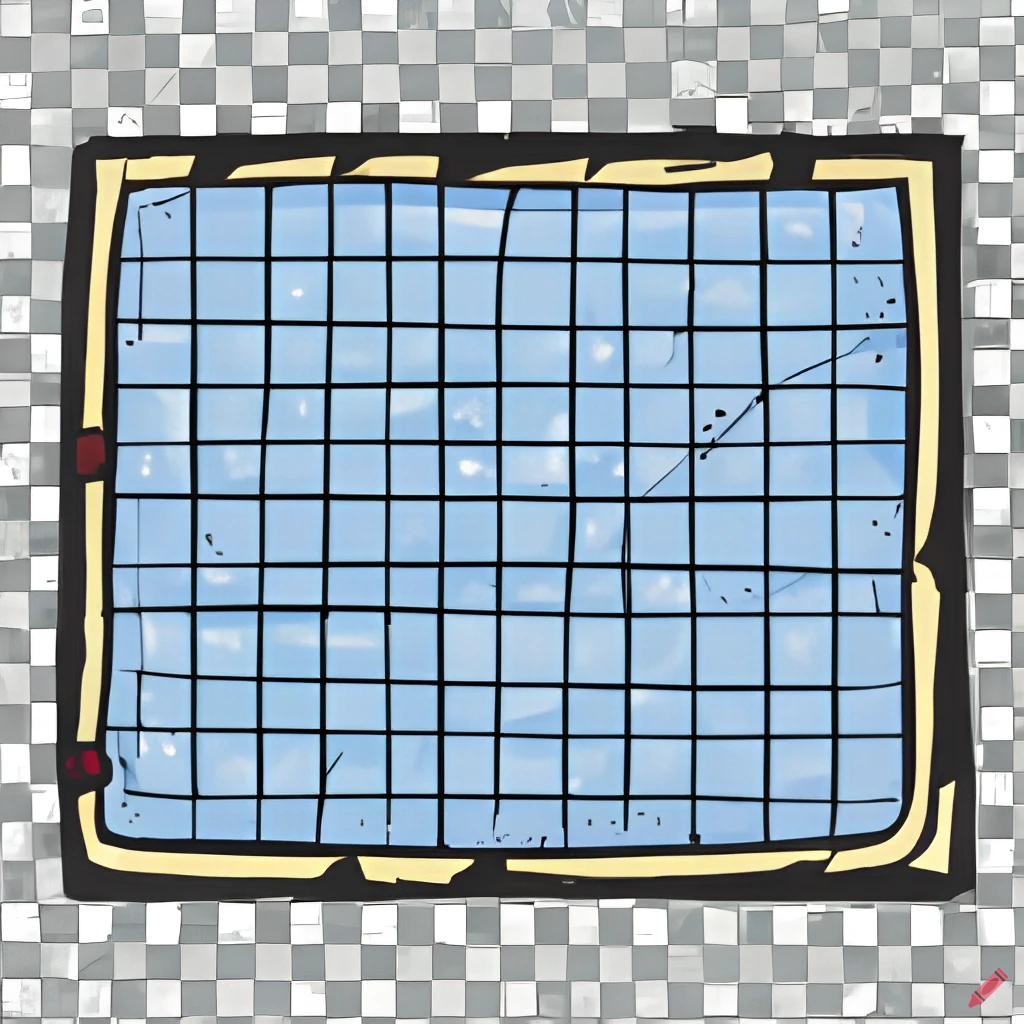
\includegraphics[width=5.5cm]{ravitaillement.jpg}
\end{wrapfigure}
Vous êtes fraichement recruté à un poste important de développement et
d'optimisation au Centre d'Activités Récréatives des Week-ends
Aventureux (CARWA). Le week-end approche à grand pas et une activité a lieu à Delft,
les équipes de candidats et de responsables sont déjà parties vers leur destination,
mais nous avons un problème, personne n'a pensé au ravitaillement !
La ville de Delft est un véritable dédale, un grand rectangle composée de zones carrées,
et il serait dangereux de laisser nos équipes sans un tel support.

Nous avons besoin de votre aide pour trouver établir la taille idéale d'un
campement de ravitaillement dans la ville sans perturber le déroulement de l'activité pour les candidats.
Vous disposez du nom de chaque équipe, leur position dans la ville et s'il s'agit d'une
équipe de candidat ou de responsables. La ville est composées de $n \times m$ petites zones carrées sur votre plan.
Les équipes de candidats ne se trouvent que sur une seule case, mais une seule équipe de responsable peut être éparpillée sur plusieurs cases.
Deux équipes ne peuvent jamais se trouver sur la même case mais une case peut être vide.

Votre but est de trouver le plus grand rectangle dans Delft où
seules des équipes de responsables se trouvent, afin qu'elles puissent créer le plus
grand camps de ravitaillement. Il doit impérativement être de forme rectangulaire, vu la complexité de se déplacer dans Delft.
Lorsque vous aurez trouvé ce rectangle, indiquez à vos supérieurs le nombre d'équipes qui seront mobilisées pour établir ce ravitaillement.

\begin{Input}
	L'entrée consiste de :
	\begin{itemize}
		\item Une ligne de trois entiers $n$, $m$ et $k$ ($1 \le n,m \le 10^3$, $1 \le k \le 20$),
respectivement le nombre de zones en ligne, le nombre de zones en colonne et le nombre d'équipes de responsables présentes sur le terrain.
		\item $n$ lignes, où une ligne contient $m$ noms séparés par un espace, c'est-à-dire de la forme $nom_1 nom_2 ... nom_m$. Le $m$\textsuperscript{ème} nom représente l'équipe sur la zone $(n,m)$,
		\item $k$ lignes, où une ligne est le nom d'une équipe de responsables.
	\end{itemize}
	Les noms sont donnés en minuscule sans caractères avec uniquement l'une des 26 lettres de l'alphabet, et lorsqu'une case n'est occupée par aucune équipe, le nom correspondant sera ``\verb|null|''.
\end{Input}

\begin{Output}
	Le nombre maximal de zones formant un rectangle dans lequel toutes les zones carrées sont occupées par des responsables.
\end{Output}
